\documentclass[conference]{IEEEtran}
\usepackage{cite}
\usepackage{amsmath,amssymb,amsfonts}
\usepackage{algorithmic}
\usepackage{graphicx}
\usepackage{textcomp}
\usepackage{xcolor}
\graphicspath{{figures/}}

\begin{document}

\title{Trade-off Analysis between Accuracy and Computational Efficiency in Sarcasm Detection Using DistilBERT and RoBERTa}

\author{\IEEEauthorblockN{Falah Razan Hibrizi}
\IEEEauthorblockA{\textit{School of Computing} \\
\textit{Telkom University}\\
Bandung, Indonesia \\
email address}
\and
\IEEEauthorblockN{Supervisor Name}
\IEEEauthorblockA{\textit{School of Computing} \\
\textit{Telkom University}\\
Bandung, Indonesia \\
email address}
}

\maketitle

\begin{abstract}
Sarcasm often expresses the opposite of its literal meaning, which causes sentiment analysis systems to misread sarcastic sentences. RoBERTa is known to be accurate but computationally expensive, whereas DistilBERT offers a smaller model. This study examines the trade-off between performance and computational efficiency of both models on 1,000,864 comment and parent comment pairs from the Self-Annotated Reddit Corpus (SARC). The comparison covers three input configurations, namely comment only, early fusion, and late fusion, as well as partial layer freezing. The final configurations were selected on validation data and locked before any test score was computed. Each configuration was run with three seeds and evaluated with the paired t-test, the Wilcoxon signed-rank test, and the Friedman test with Holm correction. The highest macro-F1 of 79.62\% was obtained by RoBERTa with early fusion, and RoBERTa outperformed DistilBERT by 1.65--2.07 points across the three inputs. Nevertheless, DistilBERT still reached 97--98\% of the RoBERTa macro-F1 while requiring only about half of the training time, latency, and GPU memory. Adding the parent comment raised macro-F1 by 0.69--1.10 points, with the largest gain on ambiguous comments. For RoBERTa, early fusion was more accurate and far cheaper than late fusion. Freezing 6 of the 12 RoBERTa layers reduced macro-F1 by only 0.24 points and cut training time by about 45\%, although inference latency did not decrease. These results indicate that RoBERTa is preferable when accuracy is the priority, whereas DistilBERT is more suitable under latency and memory constraints.
\end{abstract}

\begin{IEEEkeywords}
computational efficiency, DistilBERT, layer freezing, parent comment, RoBERTa, sarcasm detection
\end{IEEEkeywords}

\section{Introduction}
In sarcasm, the speaker says something different from, or even opposite to, what is actually meant. A compliment, for example, can be used to mock. Such sentences are difficult for sentiment analysis systems because words that look positive carry a negative intent \cite{prakash2025sarcasm}. As a result, public opinion monitoring and content moderation systems may produce wrong outputs, including when they are used to detect cyberbullying on social media \cite{dhumpati2025sarcasm}, \cite{grover2026emoji}.

The difficulty increases in written text, since there is no tone of voice or facial expression to serve as a cue \cite{jimenez2026bert}. On forums such as Reddit, the sarcastic nature of a reply often becomes clear only after the reader knows the comment being replied to, called the parent comment. The Self-Annotated Reddit Corpus (SARC) \cite{khodak2018sarc} provides a very large number of parent comment and reply pairs. Other context, such as user information and forum topic, also helps models on SARC \cite{hao2023enhanced}. Several studies on Reddit conversation data have reported that feeding the parent comment into a transformer model can improve sarcasm detection performance \cite{ataeii2020transformers}, \cite{dubey2025unpacking}.

Transformer-based models are currently widely used for this task. RoBERTa \cite{liu2019roberta} is a refinement of BERT with an improved pretraining procedure. It generally achieves high accuracy, but its memory and computation requirements are also large, while computing resources are limited \cite{treviso2023efficient}. DistilBERT \cite{sanh2019distilbert} is obtained through knowledge distillation, so it has half the layers of BERT and faster inference. Studies comparing BERT variants for sarcasm detection show that performance depends strongly on the choice of model and training settings \cite{jimenez2026bert}, \cite{ullah2026advanced}.

A direct comparison of RoBERTa and DistilBERT, including on SARC, was carried out by Dubey et al., who reported that DistilBERT trained about 1.74 times faster with competitive performance \cite{dubey2025unpacking}, \cite{dubey2026efficient}. However, both models were combined with BART context summaries and metadata embeddings, which makes it difficult to isolate the contribution of the models themselves. The experiments also used only a subset of 7,370 samples \cite{dubey2025unpacking}, and the preprocessing removed capitalization and punctuation \cite{dubey2026efficient}, even though both can signal sarcasm. In \cite{dubey2026efficient}, the performance difference between the two models was not even significant under the paired t-test ($p = 0.064$). Zhang et al.\ \cite{zhang2025enhancing} used SARC at a larger scale but did not separate test data from validation data. Meanwhile, the way the parent comment is fed into the model and layer freezing, which can serve as a cost-saving option besides distillation, have rarely been discussed together with their computational cost in the context of sarcasm detection.

Based on these observations, this study compares the performance and computational efficiency of RoBERTa and DistilBERT on approximately one million SARC comment pairs without additional components. The trade-off between the two is then analyzed to determine the conditions best suited to each model. This aim is broken down into the following three research questions.
\begin{enumerate}
\item Does the number of frozen layers affect sarcasm classification performance?
\item Does using the parent comment as input affect sarcasm classification performance?
\item Which fusion strategy yields the best sarcasm classification performance?
\end{enumerate}
The three questions are answered for both models while taking into account the computational cost in terms of training time, inference latency, GPU memory, and number of parameters. The contributions of this study are (i) a comparison of both models with light preprocessing, configurations locked before the test data were opened, three seeds, and statistical tests with Holm correction; (ii) measurements of computational cost alongside performance for three input configurations and several levels of layer freezing; and (iii) an analysis of the types of comments that benefit most from the parent comment.

\section{Methodology}

\subsection{Dataset and Preprocessing}
\label{sec:data}
This study uses the balanced version of SARC \cite{khodak2018sarc} released on Kaggle, the same version used in \cite{dubey2026efficient} and \cite{zhang2025enhancing}. It contains 1,010,826 Reddit comments together with the parent comments they reply to. The labels do not come from annotators but from the ``/s'' marker added by the comment authors themselves, and this marker was removed from the text when the corpus was built \cite{khodak2018sarc}.

Preprocessing was deliberately kept simple. In previous studies, text was lowercased, punctuation or special characters were removed, and lemmatization was applied \cite{dubey2026efficient}, \cite{zhang2025enhancing}. These steps were not applied here, because capitalization, punctuation, and emoticons such as ``;)'' may indicate sarcasm. Cleaning consisted only of decoding HTML entities, replacing Markdown links with their text, removing URLs and HTML tags, and normalizing whitespace. As a result, only 2,942 comments (0.29\%) were changed.

The number of rows removed at each step is shown in Table~\ref{tab:data}. Duplicates and conflicting labels were detected using a normalized key (lowercase and without punctuation), while the text fed to the model remained the original text. In the last step, residual artifacts of the ``/s'' marker removal were discarded. These artifacts are comments that contain only a sentence fragment, such as ``You forgot the''. They were matched with a pattern of at most eight words. Of the 8,599 matching rows, 8,580 were labeled sarcastic, so all of them were removed to prevent the model from learning this shortcut. After filtering, 1,000,864 pairs remained, with a sarcastic proportion of 49.59\%.

\begin{table}[t]
\caption{Row Filtering and Data Split}
\label{tab:data}
\centering
\begin{tabular}{lrr}
\hline
Filtering step & Removed & Remaining \\
\hline
Raw data & -- & 1,010,826 \\
Empty comment & 55 & 1,010,771 \\
Empty after cleaning & 9 & 1,010,762 \\
Conflicting labels & 142 & 1,010,620 \\
Duplicate pairs & 1,157 & 1,009,463 \\
``/s'' fragments & 8,599 & 1,000,864 \\
\hline
Split & Pairs & Sarcastic (\%) \\
\hline
Training & 799,459 & 49.66 \\
Validation & 100,276 & 49.38 \\
Test & 101,129 & 49.27 \\
\hline
\end{tabular}
\end{table}

The training, validation, and test split was performed with seed 42. The data were split by comment group rather than by row, so comments with the same key always fall into the same split. This is necessary because short replies such as ``Source?'' and ``Yes.'' appear hundreds of times in the data. The resulting split is close to an 80/10/10 ratio, and no comment or pair appears in more than one split.

\subsection{Models and Input Configurations}
RoBERTa-base \cite{liu2019roberta} consists of 12 Transformer layers with a hidden size of 768 and a total of 124.6 million parameters. DistilBERT \cite{sanh2019distilbert} is a distilled version of BERT with the same hidden size but only six layers and 65.8 million parameters. The cased version of DistilBERT was chosen so that both models can distinguish capitalization. To examine the effect of the parent comment and the fusion strategy, three input configurations were compared as follows.

\textit{Comment only.} The model receives only the reply text. This configuration serves as the baseline.

\textit{Early fusion.} The parent and comment are combined into a single input using the tokenizer's sentence-pair format, with the parent placed first. This approach is similar to the concatenation of context and response in \cite{ataeii2020transformers}. With this arrangement, every comment token can attend to all parent tokens from the first layer onward. The input length is limited to 256 tokens. When the limit is exceeded, the end of the parent is truncated, which happens for 0.85\% of the training pairs for RoBERTa and 0.99\% for DistilBERT. Comments longer than 256 tokens are also truncated, but there are only 52--54 such training comments (less than 0.01\%).

\textit{Late fusion.} The parent and comment are encoded separately with the same encoder. The final hidden states at the first token of the comment ($h_x$) and of the parent ($h_y$) are then combined into
\begin{equation}
u = [\,h_x;\; h_y;\; |h_x - h_y|;\; h_x \odot h_y\,],
\label{eq:fusion}
\end{equation}
where $[\cdot\,;\cdot]$ denotes vector concatenation and $\odot$ denotes element-wise multiplication. The vector $u$ in (\ref{eq:fusion}) is passed to the classification head, which follows the default head of each model except that its input size is four times larger. The truncation rules are the same as in early fusion. Consequently, the encoder must be run twice for every example, and comment tokens cannot attend directly to parent tokens.

\subsection{Layer Freezing}
Layer freezing is a form of selective fine-tuning because only a subset of the parameters is trained \cite{han2024peft}, and it can save GPU memory with only a small loss in accuracy \cite{ardakani2024slimfit}. In this experiment, the embedding layer and a number of the lowest layers were frozen, so that only the upper layers and the head were trained. This test was conducted on early fusion with 0, 6, 9, and 12 frozen layers out of the 12 RoBERTa layers, and 0, 3, and 6 out of the 6 DistilBERT layers. Partially frozen models were trained with three seeds using the best learning rate from full fine-tuning. For fully frozen models, learning rates of $10^{-4}$ and $10^{-3}$ were tried with seed 42, and the better one was selected on validation data. Note that freezing reduces only the training cost, because all layers are still executed during inference.

\subsection{Experimental Setup}
The training settings are summarized in Table~\ref{tab:setup}. Biases and LayerNorm parameters were excluded from weight decay, and each batch was padded only to the length of its longest sequence. The epoch with the highest validation macro-F1 was used. The learning rate was determined through a grid search because RoBERTa is known to be sensitive to training settings \cite{jimenez2026bert}. The grid includes the values $2 \times 10^{-5}$ and $3 \times 10^{-5}$ used in \cite{dubey2026efficient}, \cite{ullah2026advanced}.

\begin{table}[t]
\caption{Training Settings}
\label{tab:setup}
\centering
\begin{tabular}{ll}
\hline
Setting & Value \\
\hline
Maximum input length & 256 tokens \\
Batch size & 32 (evaluation: 128) \\
Epochs & max. 3, best by validation macro-F1 \\
Loss & cross-entropy \\
Optimizer & AdamW, weight decay 0.01 \\
Learning rate schedule & 10\% linear warm-up, then linear decay \\
Gradient clipping & 1.0 \\
Classifier dropout & 0.1 (RoBERTa), 0.2 (DistilBERT) \\
Precision & BF16 mixed precision \\
Learning rate grid (S1) & $\{1, 2, 3, 5\} \times 10^{-5}$ \\
Seeds & 42 (S1); 42, 43, 44 (final runs) \\
\hline
\multicolumn{2}{l}{Selected learning rate (RoBERTa / DistilBERT)} \\
\quad Comment only & $1 \times 10^{-5}$ / $3 \times 10^{-5}$ \\
\quad Early fusion & $2 \times 10^{-5}$ / $1 \times 10^{-5}$ \\
\quad Late fusion & $1 \times 10^{-5}$ / $1 \times 10^{-5}$ \\
\hline
\end{tabular}
\end{table}

In total, 60 runs were carried out in three scenarios: a learning rate search with seed 42 (S1, 24 runs), layer freezing (S2, 16 runs), and repetition with seeds 43 and 44 (S3, 20 runs). Of these, 29 runs were evaluated on the test data, consisting of 6 S1 runs, 11 S2 runs, and 12 S3 runs. The remaining runs either used a learning rate that lost on validation data or still used a learning rate from early trials before the learning rate search was completed (11 runs). All runs were executed on a single NVIDIA GeForce RTX 5070 Ti 16 GB GPU. Training time was computed per epoch excluding validation, and the recorded memory is the peak GPU memory during training. Latency was measured as the forward pass time with inputs already on the GPU. The measurement used 1,000 validation examples at batch sizes 1 and 32, with the first ten batches treated as an uncounted warm-up, and the results are reported per example. Efficiency figures were averaged over the same final runs that were evaluated on the test data.

\subsection{Evaluation and Statistical Testing}
\label{sec:eval}
A comment is predicted as sarcastic if its probability is 0.5 or higher. The reported metrics are accuracy, precision, recall, and F1 for the sarcastic class, plus macro-F1 as the main metric. Epoch and learning rate selection used only validation data. Test predictions were stored without being scored, and the list of 29 final runs was recorded in a manifest file committed to the project repository on 16 October 2026, before any test score was computed. Three seeds were used because the performance of neural networks can vary with the random seed \cite{ulmer2022deep}. Scores are reported as the mean and standard deviation over seeds 42, 43, and 44, except for fully frozen models, which have only one run.

All comparisons were tested with one-sided hypotheses \cite{dror2020significance}. For example, in the parent comment comparison, $H_0$ states that macro-F1 with the parent is not higher than without it, whereas $H_1$ states the opposite. The tested data are the per-seed test macro-F1 scores, paired by seed and model. Comparisons of two configurations were tested with a one-sided paired t-test. The one-sided Wilcoxon signed-rank test was added only for pooled comparisons, because with three pairs the smallest $p$-value Wilcoxon can reach is 0.125. Comparisons of three or more treatments, namely the three inputs, the three seeds, and the four learning rates, were tested with the Friedman test. Effect size is reported as the mean difference with a two-sided 95\% confidence interval (95\% CI) for two-configuration tests, and as Kendall's $W$ for the Friedman test. Normality of the differences in pooled comparisons was checked with the Shapiro-Wilk test. Given the number of tests, $p$-values were corrected with the Holm method within each question group, at a significance level of 0.05. Computational cost was tested with the same procedure. As a supporting test, run pairs were also compared at the level of individual test examples using McNemar's test with Holm correction. In addition, an exploratory analysis compared early fusion with comment only on several test subgroups, namely by comment length, comments that appear with different labels, and the confidence of the RoBERTa comment-only model. The model is considered uncertain when its mean probability lies in the range 0.4--0.6.

\section{Results}

\subsection{Performance and Efficiency of Both Models}
The test scores and computational costs of the six main configurations are presented in Table~\ref{tab:main}. The highest values on all metrics were obtained by RoBERTa with early fusion, with a macro-F1 of 79.62\%. Across the three inputs, RoBERTa outperformed DistilBERT by 1.65--2.07 points. This advantage appeared in all nine seed and input pairs. The pooled difference was 1.81 points (95\% CI 1.65--1.97) and remained significant after Holm correction (Table~\ref{tab:uji}). The results were also stable. The standard deviation of accuracy and macro-F1 did not exceed 0.09 points, the macro-F1 difference between validation and test data ranged only from $-0.07$ to 0.26 points, and the Friedman test found no difference across seeds ($p = 0.311$). Unlike the seed, the learning rate had a significant effect ($p_{\mathrm{Holm}} = 0.004$). A learning rate of $5 \times 10^{-5}$ always produced the lowest validation macro-F1, with the largest drop for RoBERTa.

\begin{table*}[t]
\caption{Test Scores and Computational Costs of the Main Configurations}
\label{tab:main}
\centering
\footnotesize
\setlength{\tabcolsep}{3pt}
\begin{tabular}{llccccccccc}
\hline
 & & \multicolumn{5}{c}{Test score (\%)} & Training & \multicolumn{2}{c}{Latency (ms)} & Memory \\
Input & Model & Accuracy & Precision & Recall & F1 & Macro-F1 & (min/epoch) & bs 1 & bs 32 & (GB) \\
\hline
Comment only & DistilBERT & 76.88 $\pm$ 0.08 & 76.94 $\pm$ 0.65 & 75.80 $\pm$ 1.17 & 76.36 $\pm$ 0.29 & 76.87 $\pm$ 0.08 & 8.56 & 4.19 & 0.15 & 2.63 \\
 & RoBERTa & 78.53 $\pm$ 0.07 & 78.33 $\pm$ 0.36 & 77.99 $\pm$ 0.46 & 78.16 $\pm$ 0.05 & 78.52 $\pm$ 0.06 & 16.61 & 8.42 & 0.31 & 5.09 \\
Early fusion & DistilBERT & 77.58 $\pm$ 0.06 & 78.14 $\pm$ 1.11 & 75.70 $\pm$ 2.03 & 76.88 $\pm$ 0.53 & 77.55 $\pm$ 0.09 & 9.93 & 4.23 & 0.32 & 2.64 \\
 & RoBERTa & \textbf{79.63} $\pm$ 0.05 & \textbf{79.37} $\pm$ 1.31 & \textbf{79.32} $\pm$ 2.22 & \textbf{79.32} $\pm$ 0.48 & \textbf{79.62} $\pm$ 0.06 & 19.03 & 8.41 & 0.61 & 5.11 \\
Late fusion & DistilBERT & 77.60 $\pm$ 0.02 & 77.62 $\pm$ 0.07 & 76.61 $\pm$ 0.07 & 77.12 $\pm$ 0.02 & 77.59 $\pm$ 0.02 & 14.92 & 7.20 & 0.42 & 4.29 \\
 & RoBERTa & 79.30 $\pm$ 0.02 & 78.82 $\pm$ 0.21 & 79.29 $\pm$ 0.39 & 79.06 $\pm$ 0.09 & 79.30 $\pm$ 0.02 & 28.82 & 15.06 & 0.83 & 8.38 \\
\hline
\multicolumn{11}{p{0.97\textwidth}}{Early and late fusion use comment + parent. Scores are mean $\pm$ standard deviation over seeds 42, 43, and 44, and costs are averaged over the same runs. Precision, recall, and F1 are computed for the sarcastic class. Latency at batch size (bs) 32 is reported per example.}
\end{tabular}
\end{table*}

In terms of efficiency, RoBERTa has 1.9 times more parameters, and its computational cost is roughly twice that of DistilBERT for all inputs. RoBERTa training took 1.92--1.94 times longer, its memory requirement was 1.93--1.96 times larger, and its batch-1 latency was 1.99--2.09 times higher. This pattern appeared consistently in all nine seed and input pairs (Wilcoxon, $p = 0.002$ for all three measures) and remained significant after Holm correction.

\begin{table}[t]
\caption{Hypothesis Test Results on Test Data}
\label{tab:uji}
\centering
\footnotesize
\setlength{\tabcolsep}{2.2pt}
\begin{tabular}{lcrcccc}
\hline
$H_1$ & $n$ & $\Delta$ & 95\% CI & $p_{\mathrm{Holm}}$ & $p_W$ & McN. \\
\hline
\multicolumn{7}{l}{\textit{Performance: RoBERTa $>$ DistilBERT}} \\
Pooled, 3 inputs & 9 & 1.81 & 1.65--1.97 & $<$0.001 & 0.002 & yes \\
\hline
\multicolumn{7}{l}{\textit{Layer freezing: full fine-tuning $>$ partially frozen}} \\
RoBERTa, 6 layers & 3 & 0.24 & $-$0.02--0.49 & 0.028 & -- & no \\
RoBERTa, 9 layers & 3 & 1.00 & 0.81--1.18 & 0.002 & -- & -- \\
DistilBERT, 3 layers & 3 & 1.47 & 1.28--1.66 & 0.002 & -- & -- \\
Pooled & 9 & 0.90 & 0.48--1.32 & 0.002 & 0.002 & -- \\
\hline
\multicolumn{7}{l}{\textit{Input: difference among the three inputs (Friedman)}} \\
Comment, early, late & 6 & \multicolumn{2}{c}{$W = 0.78$} & 0.009 & -- & -- \\
\hline
\multicolumn{7}{l}{\textit{Parent comment: comment + parent $>$ comment only}} \\
Early, RoBERTa & 3 & 1.10 & 0.83--1.37 & 0.004 & -- & yes \\
Early, DistilBERT & 3 & 0.69 & 0.65--0.72 & $<$0.001 & -- & yes \\
Late, RoBERTa & 3 & 0.78 & 0.60--0.96 & 0.004 & -- & yes \\
Late, DistilBERT & 3 & 0.72 & 0.53--0.92 & 0.004 & -- & yes \\
Early, pooled & 6 & 0.89 & 0.64--1.14 & $<$0.001 & 0.016 & -- \\
Late, pooled & 6 & 0.75 & 0.67--0.83 & $<$0.001 & 0.016 & -- \\
\hline
\multicolumn{7}{l}{\textit{Fusion strategy: early fusion $>$ late fusion}} \\
RoBERTa & 3 & 0.32 & 0.15--0.49 & 0.023 & -- & yes \\
DistilBERT & 3 & $-$0.04 & $-$0.26--0.19 & 0.725 & -- & no \\
Pooled & 6 & 0.14 & $-$0.08--0.36 & 0.158 & 0.109 & -- \\
\hline
\multicolumn{7}{l}{\textit{Cost: RoBERTa $>$ DistilBERT (pooled, 3 inputs)}} \\
Training (min/epoch) & 9 & 10.35 & 8.27--12.43 & $<$0.001 & 0.002 & -- \\
Latency bs 1 (ms) & 9 & 5.42 & 4.01--6.82 & $<$0.001 & 0.002 & -- \\
Memory (GB) & 9 & 3.01 & 2.38--3.64 & $<$0.001 & 0.002 & -- \\
\hline
\multicolumn{7}{l}{\textit{Supporting (Friedman)}} \\
Three seeds & 6 & \multicolumn{2}{c}{$W = 0.19$} & 0.311 & -- & -- \\
Learning rate (validation) & 6 & \multicolumn{2}{c}{$W = 0.74$} & 0.004 & -- & -- \\
\hline
\multicolumn{7}{p{0.95\columnwidth}}{$n$: number of pairs or blocks; $\Delta$: mean difference (macro-F1 points, or cost units); 95\% CI: two-sided, so it may slightly include zero even when the one-sided test is significant; $p_{\mathrm{Holm}}$: paired t-test or Friedman $p$ after Holm correction within each question group; $p_W$: Wilcoxon; McN.: significant under McNemar with Holm correction for all three seeds (--: not tested).}
\end{tabular}
\end{table}

\subsection{Effect of the Number of Frozen Layers}
Fig.~\ref{fig:frozen} shows macro-F1 and training time for each number of frozen layers. When 6 of the 12 RoBERTa layers were frozen, macro-F1 dropped only from 79.62\% to 79.38\%. This 0.24-point drop occurred in all three seeds and was significant under the one-sided paired t-test ($p_{\mathrm{Holm}} = 0.028$), with a one-sided 95\% CI lower bound of 0.07 points. However, the two-sided 95\% CI ($-0.02$--0.49) still slightly crosses zero and McNemar did not find it significant, so the drop can be considered small. On the cost side, training time fell from 19.03 to 10.51 min per epoch, and memory fell from 5.11 to 2.70 GB. With 9 frozen layers, RoBERTa still reached 78.62\%. This is 1.07 points higher than fully fine-tuned DistilBERT, even though its training time was shorter (7.49 vs.\ 9.93 min) and its memory was smaller (1.67 vs.\ 2.64 GB). DistilBERT turned out to be more sensitive to freezing, as freezing only 3 of its 6 layers already reduced macro-F1 by 1.47 points. When all layers were frozen, macro-F1 of both models fell to around 65\%. Latency remained relatively unchanged, at 7.80--8.41 ms for RoBERTa and 3.91--4.23 ms for DistilBERT, and the latency reduction due to freezing was not significant after Holm correction ($p_{\mathrm{Holm}} = 0.079$).

\begin{figure}[t]
\centering
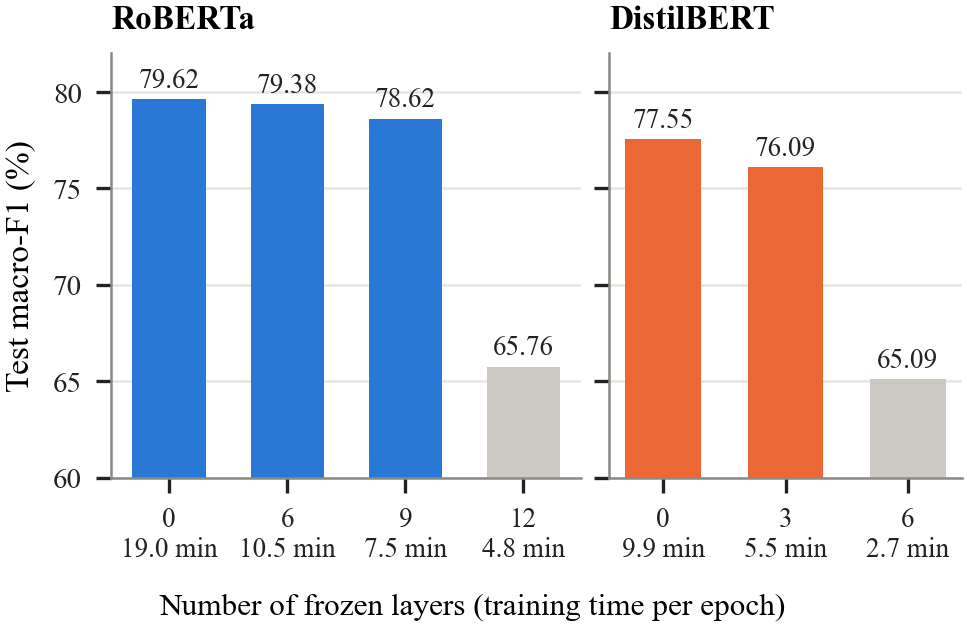
\includegraphics[width=\columnwidth]{fig_frozen_layers_en}
\caption{Test macro-F1 by number of frozen layers in early fusion. The numbers below the axis show the training time per epoch. Grey bars are fully frozen models (one seed); the other bars are means over three seeds.}
\label{fig:frozen}
\end{figure}

\subsection{Effect of the Parent Comment}
The Friedman test showed a difference in macro-F1 among the three inputs ($p = 0.009$, Kendall's $W = 0.78$). As shown in Fig.~\ref{fig:input}, adding the parent increased macro-F1 for both models. With early fusion, the gain was 1.10 points for RoBERTa and 0.69 points for DistilBERT, while late fusion gave gains of 0.78 and 0.72 points. All four gains were significant, both under the paired t-test after Holm correction and under McNemar. The additional cost of early fusion was small. Training time increased by only 1.15--1.16 times, while batch-1 latency and memory barely changed. Only the per-example latency at batch size 32 increased to roughly twice.

\begin{figure}[t]
\centering
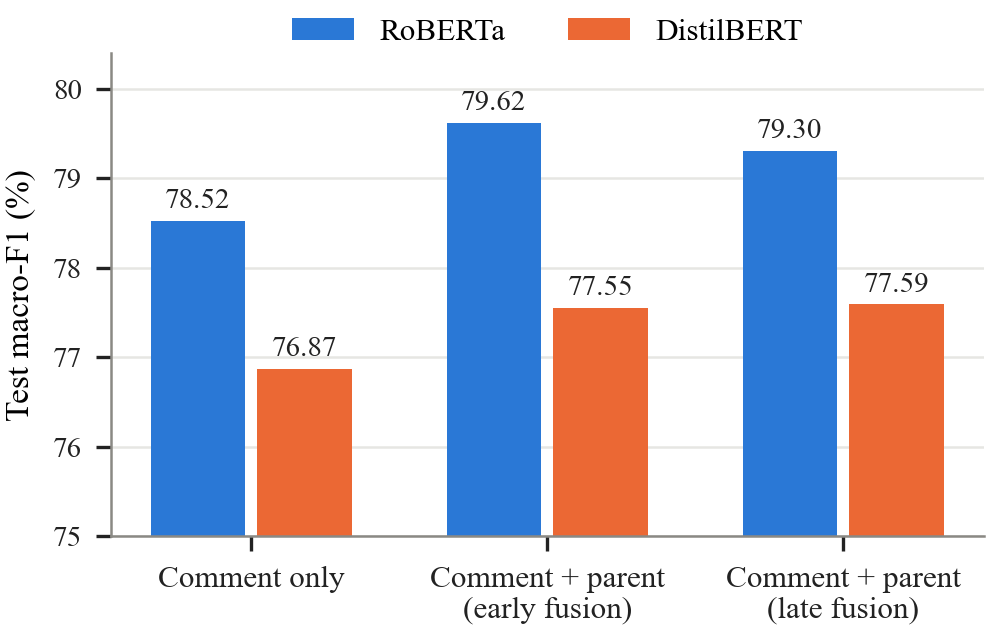
\includegraphics[width=\columnwidth]{fig_macro_f1_input_en}
\caption{Test macro-F1 for each model and input configuration (mean over three seeds). The vertical axis starts at 75\% so that differences between configurations are visible.}
\label{fig:input}
\end{figure}

The benefit of the parent was not uniform across comments. On the 10,737 comments for which the RoBERTa comment-only model was uncertain, early fusion increased RoBERTa macro-F1 by 8.18 points, whereas on confidently predicted comments the gain was only 0.25 points. The gain on short comments of 1--3 words (2.59 points) was also larger than on comments longer than 10 words (0.71 points). On the 5,886 comments (593 unique sentences) that appear with different labels, the gain reached 2.73 points. Even so, the parent did not always help. For RoBERTa, the parent corrected an average of 6,236 predictions per seed but also turned 5,119 other predictions wrong.

\subsection{Best Fusion Strategy}
For RoBERTa, early fusion produced the highest macro-F1 and outperformed late fusion by 0.32 points (95\% CI 0.15--0.49, $p_{\mathrm{Holm}} = 0.023$). This result was also significant under McNemar. For DistilBERT, the two strategies gave equivalent results (77.55\% and 77.59\%). When both models were pooled, the advantage of early fusion was not significant ($p_{\mathrm{Holm}} = 0.158$, 95\% CI $-0.08$--0.36). In terms of cost, late fusion was the most expensive configuration, with about 1.5 times the training time, 1.62--1.64 times the memory, and 1.70--1.79 times the batch-1 latency of early fusion.

\section{Discussion}

\subsection{Trade-off between RoBERTa and DistilBERT}
The test results provide statistical evidence that RoBERTa is more accurate. However, its advantage is only 1.65--2.07 points, while its cost is about twice that of DistilBERT. In other words, DistilBERT retains 97--98\% of the RoBERTa macro-F1 with roughly half the resources. This cost ratio is nearly the same for all three inputs, so it is most likely determined by model size. RoBERTa is more suitable when accuracy is the priority and resources are available, for example in offline analysis. Conversely, DistilBERT is more suitable when latency and memory are limited, such as in moderation tools that must process comments continuously.

\subsection{Layer Freezing and Distillation}
The test results support an effect of the number of frozen layers on performance, although the effect is not linear. Freezing half of the RoBERTa layers reduced macro-F1 by only 0.24 points, while training time fell by 45\% and memory by 47\%, in line with \cite{ardakani2024slimfit}. A clear drop appeared only at 9 layers and became very large when all layers were frozen, so the pretrained representations still need to be fine-tuned. DistilBERT performance dropped faster, probably because it has fewer layers. In addition, freezing and distillation save different parts of the cost. Freezing saves only training cost and therefore suits models that need frequent retraining, whereas DistilBERT saves inference cost because its latency is about half that of RoBERTa.

\subsection{Role of the Parent Comment}
The test results provide statistical evidence that the parent comment improves the performance of both models, although the average gain is only about one point. This small gain is reasonable, since most comments can already be understood from their own content. The parent matters mainly when a comment is ambiguous. An example is the reply ``;)'', which appears 68 times in the test data, of which only six are sarcastic. As a reply to ``Sarcasm doesn't translate well through text. Haha'', this comment is labeled sarcastic, whereas as a reply to ``What is your Guilty Pleasure?'', the same comment is not sarcastic. Without the parent, the model must give the same prediction for both. The gain obtained here is much smaller than that reported by Dubey et al.\ (7.1 points \cite{dubey2026efficient} and 6.8 points \cite{dubey2025unpacking}), who used a subset of 7,370 samples with punctuation and capitalization removed. A comment-only model without punctuation may rely more on the parent, but this hypothesis was not tested in this study.

\subsection{Early Fusion and Late Fusion}
Early fusion was chosen as the best strategy because there is statistical evidence that it is more accurate for RoBERTa, it is not significantly different for DistilBERT, and its cost is much lower. In early fusion, comment tokens can attend to specific words in the parent at every layer. In late fusion, by contrast, both texts are first compressed into a single vector each and only meet at the classification head. Since the meaning of sarcasm is often determined by specific phrases in the parent, late fusion appears to be less advantageous. Late fusion may still be useful when one parent receives many replies, because the parent vector needs to be computed only once, but this scenario was not tested.

\subsection{Comparison with Other Studies and Limitations}
Several studies have reported higher scores, for example an F1 of 95.6\% in \cite{dubey2026efficient} and 0.917 in \cite{zhang2025enhancing}. However, the data size, preprocessing, and evaluation protocol in those studies differ. The ``/s'' fragments described in Section~\ref{sec:data} may also play a role, because almost all of them are labeled sarcastic, while none of the cited reports state whether such fragments were removed. The cost ratio, on the other hand, is consistent: the RoBERTa training time on SARC in \cite{dubey2026efficient} is 1.76 times that of DistilBERT (8.1 and 4.6 hours), compared with 1.92--1.94 times in this study.

The answers to the three research questions apply only to the dataset and settings used, with several limitations. First, training was limited to three epochs, even though 24 of the 29 final runs reached their best validation score at the last epoch. Second, only one dataset was used, and its labels come from the ``/s'' marker, so sarcastic comments without the marker are recorded as non-sarcastic \cite{khodak2018sarc}. The official SARC test split also could not be used because its text is not available. Third, the frozen models used the learning rate from full fine-tuning, the fully frozen models were run with only one seed, and each per-configuration test had only three pairs. Finally, large language models were not included, and all efficiency measurements were performed on a single GPU.

\section{Conclusion}
This study examined the trade-off between performance and computational efficiency of RoBERTa and DistilBERT for sarcasm detection on SARC. The test results provide statistical evidence that RoBERTa is more accurate, but its advantage is only about two macro-F1 points, while its computational cost is roughly twice that of DistilBERT. The number of frozen layers affects performance, but half of the RoBERTa layers can still be frozen with a very small drop to save training cost. Adding the parent comment improves the performance of both models, and early fusion is the best strategy because it is the most accurate for RoBERTa and cheaper than late fusion. Therefore, RoBERTa with early fusion is recommended when accuracy is the priority, whereas DistilBERT with early fusion is recommended when latency and memory are limited. Future work could extend training, search for learning rates specific to frozen models, test other datasets, and compare the results with large language models.

\bibliographystyle{IEEEtran}
\bibliography{references}

\end{document}
